\documentclass[11pt]{article}

\usepackage[margin=1.1in]{geometry}
\usepackage{amsmath,amssymb,amsthm}
\usepackage{graphicx}
\usepackage{booktabs}
\usepackage{microtype}
\usepackage{xcolor}
\usepackage{tikz}
\usepackage[colorlinks=true,linkcolor=blue!60!black,citecolor=blue!60!black,urlcolor=blue!60!black]{hyperref}
\usepackage{caption}
\captionsetup{font=small,labelfont=bf}

\graphicspath{{figures/}}

\newtheorem{theorem}{Theorem}
\newcommand{\lplus}{\lambda_{+}}
\newcommand{\lminus}{\lambda_{-}}
\newcommand{\tr}{\operatorname{tr}}
\newcommand{\Imag}{\operatorname{Im}}

\title{From Wigner's Surmise to the Marchenko--Pastur Law:\\
An Account of Random Matrix Theory,\\
with an Application to NSE Equity Portfolios}

% TODO: confirm author name and affiliation before submission
\author{Riwa Desai}
\date{July 2026}

\begin{document}
\maketitle

\begin{abstract}
This paper is an expository account of the random matrix theory I have
studied, organized as the subject itself unfolded: what a random matrix is, the two inequivalent ways a matrix ensemble can
be structureless---independent entries, or rotational invariance---and the
proof, by a two-by-two trace computation, that the Gaussian ensembles (GOE,
GUE) are exactly where the two properties meet; Wigner's surmise for the
spacing of adjacent eigenvalues, including the calculation from which it
takes its name; the Wishart ensemble, which is what a random matrix looks
like when it arises as a sample covariance matrix; and the
Marchenko--Pastur theorem, the spectral law of Wishart matrices, derived
here in full using the Stieltjes transform and its
inversion formula, the Sherman--Morrison rank-one update, Sylvester's
determinant identity, and the concentration of quadratic forms---with a
careful discussion of why the theorem lives in the limit where both matrix
dimensions diverge at a fixed ratio $\gamma=N/T$. The final part puts the
theory to work on data I assembled: daily returns of $548$ National Stock
Exchange of India equities over $1236$ trading days. The eigenvalue bulk of
the sample correlation matrix matches the Marchenko--Pastur density, its
level spacings match Wigner's surmise (and decisively reject the Poisson
alternative), and a covariance matrix cleaned by flattening the noise band
delivers out-of-sample minimum-variance portfolios with 7.8\% annualized
volatility against 9.3\% for Ledoit--Wolf shrinkage, 17.7\% for equal
weights, and 19.4\% for the raw matrix. Nothing in the theory below is new;
the aim is to show, end to end, how these classical results connect and
what they can do when applied carefully.
\end{abstract}

\section*{Acknowledgements}

This paper is a record of self-study, and its debts are to teachers I
have never met. The \emph{Linear Algebra} and \emph{Abstract Linear
Algebra} playlists of the YouTube channel \textbf{The Bright Side of
Mathematics} built the foundations on which everything here stands.
\textbf{Roland Speicher}'s lecture playlist on high-dimensional random
matrices taught me how the subject thinks in the large-$N$ limit.
\textbf{Euler Bernhard}'s \emph{Random Matrices: Theory and Practice}
playlist walked me through the ensembles and their spectral laws with
exactly the mix of rigor and intuition I have tried to reproduce in
Sections~\ref{sec:wigner}--\ref{sec:derivation}. And \textbf{Terence
Tao}'s writing on random matrix theory showed me what it looks like when
deep mathematics is explained with total clarity. Any errors of
understanding in these pages are, of course, entirely my own.

\section{Introduction}
\label{sec:intro}

This is not a research paper in the usual sense. It is a record of
understanding: an attempt to lay out, in one connected narrative, a body of
classical mathematics I have studied---random matrix theory, from Wigner's
work in the 1950s to the Marchenko--Pastur theorem of 1967---and then to
show that the understanding is real by applying it to a concrete problem:
estimating the covariance matrix of Indian equities well enough
to build portfolios that survive contact with unseen data.

The narrative has a natural arc, and the paper follows it.
Section~\ref{sec:rmt} explains what random matrix theory is and the
physical question that created it. Section~\ref{sec:wigner} maps the
landscape of ensembles---matrices with \emph{independent entries} on one
side, \emph{rotationally invariant} ensembles on the other, and the
Gaussian ensembles (GOE, GUE, GSE) living precisely in their
intersection, a fact proved by a short trace computation that was the
first genuine proof I learned in this subject---and then presents Wigner's
surmise for eigenvalue spacings, with the two-by-two calculation behind
it. Section~\ref{sec:wishart} explains
why finance forces a different ensemble: covariance matrices are not
symmetric matrices with independent entries but matrices of the form
$X^{\top}X$, whose ensemble is Wishart's and whose spectral law is
Marchenko--Pastur's.
Section~\ref{sec:derivation} is the heart of the paper: a complete
derivation of the Marchenko--Pastur density from the Wishart setup, built
from four tools---the Stieltjes transform and its inversion, the
Sherman--Morrison update, Sylvester's determinant identity, and
concentration of quadratic forms---each stated and proved or sketched
before it is used, together with an explanation of why the limit is taken
with both dimensions growing at fixed ratio. Section~\ref{sec:application}
then applies everything at once to five years of NSE data, testing the
claim that the in-band eigenvalues are genuinely noise in three layers of
increasing strictness: the Marchenko--Pastur density confirms they are
\emph{distributed} like noise, Wigner's surmise confirms they
\emph{interact} like noise, and an out-of-sample portfolio backtest---in
which discarding the band's contents was free to backfire---confirms they
\emph{price} like noise, beating the raw matrix, Ledoit--Wolf shrinkage,
and equal weights decisively. Section~\ref{sec:conclusion} reflects on
what the exercise taught.

Everything in Sections~\ref{sec:rmt}--\ref{sec:derivation} is classical
material, drawn from the literature
\cite{wigner1958,mehta2004,marchenko1967,baisilverstein2010,bun2017}; the
data work in Section~\ref{sec:application} is my own, in the tradition
started for financial correlation matrices by Laloux et al.\
\cite{laloux1999} and Plerou et al.\ \cite{plerou2002}.

\section{What random matrix theory is}
\label{sec:rmt}

Random matrix theory begins with a confession of ignorance. In the 1950s,
Eugene Wigner faced nuclear energy spectra too complicated to compute from
first principles, and made a radical move: model the unknown system as a
matrix with \emph{random} entries, constrained only by basic symmetry, and
ask what its eigenvalues look like \emph{typically}. The gamble was that
quantities like the spectrum's shape and the gaps between neighbouring
levels don't depend on microscopic detail at all---that they are
\emph{universal}---so a maximally ignorant model predicts them correctly.
The gamble won: level statistics across nuclei, atoms, and chaotic quantum
systems of every kind match the random-matrix predictions, and the same
universality later turned out to govern systems with no physics at all,
from traffic flow to financial correlations.

The canonical model is the \emph{Gaussian Orthogonal Ensemble} (GOE): a
real symmetric $N\times N$ matrix $H$ whose entries on and above the
diagonal are independent Gaussians, $H_{ii}\sim\mathcal{N}(0,1)$ and
$H_{ij}\sim\mathcal{N}(0,\tfrac{1}{2})$ for $i<j$. (The variance convention
makes the distribution invariant under every orthogonal change of basis
$H\mapsto O^{\top}HO$---``no basis is special,'' the mathematical form of
maximal ignorance.) As $N$ grows, what do the eigenvalues
$\lambda_1,\dots,\lambda_N$ of such a matrix do?

Two kinds of answer exist, and the distinction organizes everything that
follows. \emph{Global} statistics describe where the eigenvalues lie on
average---the limiting histogram, or spectral density. \emph{Local}
statistics describe how neighbouring eigenvalues space themselves---whether
they cluster, ignore each other, or repel. For the covariance matrices of
finance, the global answer is the Marchenko--Pastur law derived in
Section~\ref{sec:derivation}; the local answer, which universality makes
common to essentially all of these ensembles, is Wigner's surmise. Before
either, we should understand the ensembles themselves.

\section{The Gaussian ensembles, and Wigner's surmise}
\label{sec:wigner}

\subsection{Two ways to be structureless, and where they meet}
\label{sec:ensembles}

\begin{figure}[t]
\centering
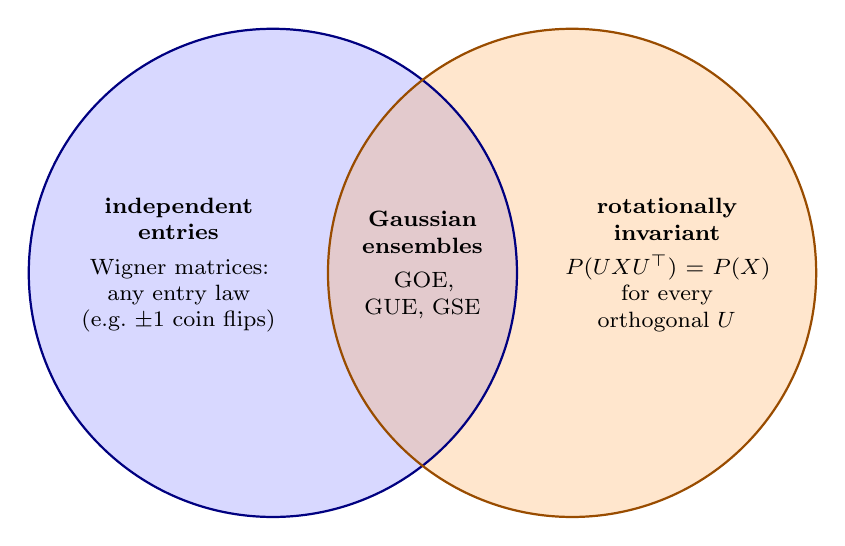
\begin{tikzpicture}
  \begin{scope}[opacity=0.28]
    \fill[blue!55]   (-1.9,0) circle (3.1);
    \fill[orange!70] ( 1.9,0) circle (3.1);
  \end{scope}
  \draw[thick, blue!50!black]   (-1.9,0) circle (3.1);
  \draw[thick, orange!60!black] ( 1.9,0) circle (3.1);
  \node[align=center, font=\footnotesize, text width=2.9cm] at (-3.1,0.1)
    {\textbf{independent entries}\\[3pt] Wigner matrices:\\ any entry law\\ (e.g.\ $\pm1$ coin flips)};
  \node[align=center, font=\footnotesize, text width=2.9cm] at ( 3.1,0.1)
    {\textbf{rotationally invariant}\\[3pt] $P(UXU^{\top})=P(X)$\\ for every\\ orthogonal $U$};
  \node[align=center, font=\footnotesize, text width=1.7cm] at (0,0.1)
    {\textbf{Gaussian ensembles}\\[3pt] GOE, GUE, GSE};
\end{tikzpicture}
\caption{The landscape of random matrix ensembles. One can demand
statistical structurelessness (independent entries) or geometric
structurelessness (no preferred basis). The two demands are genuinely
different---and the Gaussian ensembles are, essentially uniquely, where
they meet.}
\label{fig:venn}
\end{figure}

A random matrix model must decide what ``no structure'' means, and there
are two natural, inequivalent answers (Figure~\ref{fig:venn}). The first
is \emph{statistical}: fill the matrix with \textbf{independent entries},
of whatever distribution---Gaussians, coin flips, fat-tailed returns.
Matrices of this kind (symmetric, with independent entries above the
diagonal) are called \emph{Wigner matrices}. The second is
\emph{geometric}: demand that the ensemble have \textbf{no preferred
basis}, i.e.\ that the probability density be \emph{rotationally
invariant},
\[
P(UXU^{\top})=P(X)\qquad\text{for every orthogonal }U,
\]
so that the model looks identical in every coordinate system---the
mathematical form of Wigner's ``maximal ignorance.'' These two demands
are genuinely different. A symmetric matrix of independent $\pm1$ coin
flips is a perfectly good Wigner matrix, but rotating it produces entries
that are neither $\pm1$ nor independent; conversely, a typical invariant
ensemble has correlated entries. Neither set contains the other.

The remarkable fact is that the intersection is essentially a single
point: the \emph{Gaussian} ensembles, and nothing else \cite{mehta2004}.
I found the direct verification more illuminating than the abstract
statement, so here it is for the $2\times2$ real symmetric case. Take
\[
X=\begin{pmatrix} x_1 & x_3\\ x_3 & x_2\end{pmatrix},
\qquad
x_1,x_2\sim\mathcal N(0,1),\quad x_3\sim\mathcal N(0,\tfrac12),
\]
all independent. The joint density is the product of the three marginals,
\[
P(X)=P(x_1)P(x_2)P(x_3)
=\frac{1}{\sqrt{2\pi}}\cdot\frac{1}{\sqrt{2\pi}}\cdot\frac{1}{\sqrt{\pi}}
\;e^{-\frac12 x_1^{2}-\frac12 x_2^{2}-x_3^{2}}
=\frac{1}{2\pi\sqrt{\pi}}\;
e^{-\frac12\left(x_1^{2}+x_2^{2}+2x_3^{2}\right)}.
\]
Now compute $X^{2}$: its diagonal entries are $x_1^{2}+x_3^{2}$ and
$x_2^{2}+x_3^{2}$, so
\[
\tr X^{2}=x_1^{2}+x_2^{2}+2x_3^{2},
\]
exactly the combination in the exponent. The three independent marginals
have conspired to produce a density that depends on the matrix only
through a trace:
\begin{equation}
P(X)=\frac{1}{2\pi\sqrt{\pi}}\;e^{-\frac12\tr X^{2}}.
\label{eq:goe-density}
\end{equation}
Rotational invariance is now immediate: for any orthogonal $U$,
\[
\tr\!\left[(UXU^{\top})^{2}\right]
=\tr\!\left[UX^{2}U^{\top}\right]
=\tr X^{2}
\]
by cyclicity of the trace, so $P(UXU^{\top})=P(X)$ (and the volume
element $dX$ is likewise invariant, orthogonal conjugation being an
isometry). Independence of the entries was manifest by construction;
invariance fell out of the trace. This is the GOE, sitting in the
intersection of the two circles---and the same computation runs in
reverse: demanding \emph{both} properties forces the exponent to be built
from $\tr X$ and $\tr X^{2}$ alone, i.e.\ forces Gaussian entries. At
general $N$ nothing changes:
$\tr X^{2}=\sum_i x_{ii}^{2}+2\sum_{i<j}x_{ij}^{2}$, so
Eq.~\eqref{eq:goe-density} still factorizes entry by entry (independence)
while depending only on a trace (invariance).

Why the \emph{orthogonal} group specifically? Because a real symmetric
matrix is diagonalized by an orthogonal matrix (the spectral theorem):
the invariance group of the ensemble matches the group that diagonalizes
its members. The consequence is worth internalizing---in a rotationally
invariant ensemble the eigenvectors carry no information at all, and
\emph{everything} statistical lives in the eigenvalues. The family has
two siblings, indexed by Dyson's $\beta$: complex Hermitian matrices with
independent complex-Gaussian entries, invariant under \emph{unitary}
conjugation $P(UXU^{\dagger})=P(X)$, form the GUE ($\beta=2$, the
relevant ensemble when time-reversal symmetry is broken); quaternionic
self-dual matrices with symplectic invariance form the GSE ($\beta=4$).
The GOE ($\beta=1$) is the one that matches real, time-reversal-symmetric
problems---and real-valued data matrices, which is why it is the right
reference point for what follows. (The GOE also has a celebrated global
law of its own, Wigner's semicircle \cite{wigner1958}; we will not need
it, because the global law relevant to covariance matrices is
Marchenko--Pastur's, derived in Section~\ref{sec:derivation}.)

\subsection{The local answer: Wigner's surmise}
\label{sec:surmise}

The subtler question is local: take two \emph{adjacent} eigenvalues,
$\lambda_{i}$ and $\lambda_{i+1}$, and let $s$ be their spacing measured in
units of the mean spacing. What is the distribution of $s$? If eigenvalues
ignored one another---if they behaved like independent uniform points, a
Poisson process---the answer would be
\begin{equation}
P_{\mathrm{Poisson}}(s)=e^{-s},
\end{equation}
which is \emph{largest} at $s=0$: independent points love to clump.
Wigner's surmise is that GOE eigenvalues do the opposite:
\begin{equation}
P_{\mathrm{W}}(s)=\frac{\pi s}{2}\,e^{-\pi s^{2}/4},
\label{eq:surmise}
\end{equation}
which \emph{vanishes} at $s=0$. Eigenvalues of a random symmetric matrix
repel: finding two of them nearly degenerate is not merely rare but
suppressed linearly in their distance. This \emph{level repulsion} is the
sharpest fingerprint of random-matrix behaviour, and it is the second test
we will apply to financial data.

The name ``surmise'' has a story worth telling, because the calculation
behind it is the most instructive small proof in the subject. Asked at a
1956 conference what the spacing distribution of a large random matrix
should be, Wigner guessed that the answer for $N\to\infty$ would be close
to the answer for the smallest nontrivial case, $N=2$---which can be
computed exactly. Return to the $2\times2$ GOE matrix of
Section~\ref{sec:ensembles}, with its density
Eq.~\eqref{eq:goe-density}. Its two eigenvalues are
\[
\lambda_{2,1}=\frac{x_1+x_2}{2}\pm\frac12\sqrt{(x_1-x_2)^{2}+4x_3^{2}},
\]
so the spacing $s=\lambda_2-\lambda_1$ is
\[
s=\sqrt{(x_1-x_2)^{2}+4x_3^{2}},
\]
and its distribution is the density of Section~\ref{sec:ensembles}
integrated over the surface where the spacing equals $s$:
\begin{equation}
P(s)=\int\!\!\int\!\!\int
\frac{dx_1}{\sqrt{2\pi}}\,\frac{dx_2}{\sqrt{2\pi}}\,\frac{dx_3}{\sqrt{\pi}}
\;e^{-\frac12\left(x_1^{2}+x_2^{2}+2x_3^{2}\right)}\;
\delta\!\left(s-\sqrt{(x_1-x_2)^{2}+4x_3^{2}}\right).
\label{eq:ps-integral}
\end{equation}
The square root begs for polar-type coordinates. Change variables from
$(x_1,x_2,x_3)$ to $(r,\theta,\psi)$:
\[
x_1-x_2=r\cos\theta,\qquad 2x_3=r\sin\theta,\qquad x_1+x_2=\psi,
\]
that is,
\[
x_1=\frac{\psi+r\cos\theta}{2},\qquad
x_2=\frac{\psi-r\cos\theta}{2},\qquad
x_3=\frac{r}{2}\sin\theta,
\]
under which the spacing becomes simply
$s=\sqrt{r^{2}\cos^{2}\theta+r^{2}\sin^{2}\theta}=r$. The change of
measure is the $3\times3$ Jacobian
\[
J=
\begin{pmatrix}
\dfrac{\partial x_1}{\partial r} & \dfrac{\partial x_1}{\partial\theta} & \dfrac{\partial x_1}{\partial\psi}\\[8pt]
\dfrac{\partial x_2}{\partial r} & \dfrac{\partial x_2}{\partial\theta} & \dfrac{\partial x_2}{\partial\psi}\\[8pt]
\dfrac{\partial x_3}{\partial r} & \dfrac{\partial x_3}{\partial\theta} & \dfrac{\partial x_3}{\partial\psi}
\end{pmatrix}
=
\begin{pmatrix}
\dfrac{\cos\theta}{2} & -\dfrac{r\sin\theta}{2} & \dfrac12\\[8pt]
-\dfrac{\cos\theta}{2} & \dfrac{r\sin\theta}{2} & \dfrac12\\[8pt]
\dfrac{\sin\theta}{2} & \dfrac{r\cos\theta}{2} & 0
\end{pmatrix},
\]
whose determinant (expand along the third column, and watch the two
cofactors conspire) is
\[
\det J=-\frac r4,
\qquad\text{so}\qquad
dx_1\,dx_2\,dx_3=\frac r4\,dr\,d\theta\,d\psi .
\]
The exponent transforms just as cooperatively:
\[
x_1^{2}+x_2^{2}+2x_3^{2}
=\frac{(\psi+r\cos\theta)^{2}+(\psi-r\cos\theta)^{2}}{4}
+\frac{r^{2}\sin^{2}\theta}{2}
=\frac{\psi^{2}+r^{2}}{2},
\]
with all $\theta$-dependence cancelling. Equation~\eqref{eq:ps-integral}
now factorizes completely: the delta function sets $r=s$, the angle
integrates to $2\pi$, and the centre-of-mass variable $\psi$ integrates to
a Gaussian constant $\int e^{-\psi^{2}/4}d\psi=2\sqrt\pi$:
\[
P(s)=\frac{1}{2\pi\sqrt\pi}\cdot\frac{s}{4}\,e^{-s^{2}/4}
\cdot 2\pi\cdot 2\sqrt\pi
=\frac{s}{2}\,e^{-s^{2}/4}.
\]
This is the exact spacing density of the $2\times2$ Gaussian matrix. The
factor $s$---the level repulsion---came from the Jacobian: it is the polar
area element, and its origin is geometric. For the spacing to vanish,
\emph{two} independent quantities ($x_1-x_2$ and $2x_3$, the two Cartesian
components of $r$) must vanish simultaneously; degeneracy is a
codimension-two event, and the area available at radius $r$ shrinks
linearly as $r\to0$. Eigenvalues repel because degeneracies are corners in
a space where randomness has room to turn. Finally, the mean of
$\frac s2 e^{-s^{2}/4}$ is $\sqrt\pi$; measuring the spacing in units of
its mean ($s\to s/\sqrt\pi$) turns the result into
Eq.~\eqref{eq:surmise}. Wigner's guess---that $N=2$ already captures
$N=\infty$---turned out accurate to about one percent, which is why a
one-page calculation still carries the name of a theorem.

\begin{figure}[t]
\centering
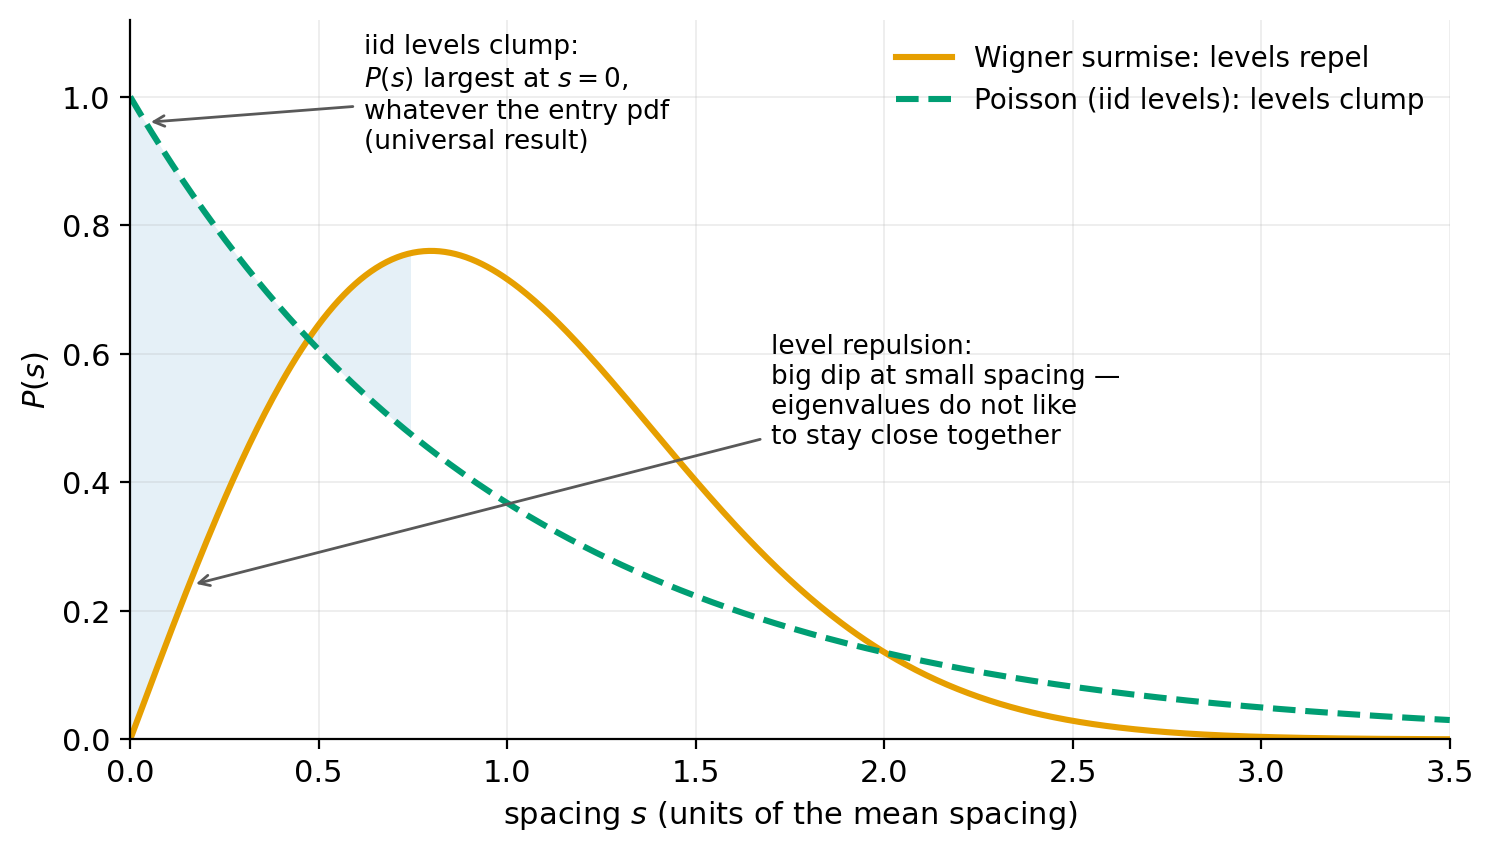
\includegraphics[width=0.82\textwidth]{fig_surmise_vs_poisson.png}
\caption{The two competing spacing laws, redrawn from my study notes.
Independent (Poisson) levels clump: whatever the pdf of the individual
levels, the probability of finding two of them very close together is
\emph{largest}---a universal result. Wigner--Dyson levels repel: the
surmise vanishes linearly at $s=0$, the ``big dip'' at small spacing.
Poisson is the statistics of things that ignore each other; Wigner--Dyson
is the statistics of things that repel. Which of the two describes the
eigenvalues of a financial correlation matrix is an empirical
question---answered in Section~\ref{sec:application}.}
\label{fig:surmise}
\end{figure}

Figure~\ref{fig:surmise} draws the two laws side by side. Everything that
matters is at the origin: independent levels pile up there, repelling
levels dig a hole. When we meet real data in
Section~\ref{sec:application}, this contrast is what makes the spacing
histogram such a sharp diagnostic---no fitted parameter can move a pile-up
into a hole.

\section{From symmetric matrices to Wishart matrices}
\label{sec:wishart}

Finance hands us a random matrix of a different shape. Collect daily
returns of $N$ stocks over $T$ days into $X\in\mathbb R^{T\times N}$ (row
$t$ = the market on day $t$), standardize each column, and form the sample
correlation matrix
\begin{equation}
S=\frac{1}{T}X^{\top}X.
\label{eq:S}
\end{equation}
This matrix is symmetric, but it is emphatically \emph{not} a GOE matrix:
its entries are strongly dependent (all built from the same $X$), it is
positive semidefinite by construction, and its natural null model is not
``ignorant Hamiltonian'' but ``returns with no true correlations at
all''---$X$ filled with i.i.d.\ noise of variance $\sigma^{2}$. When the
noise is Gaussian, $TS$ is the \emph{Wishart ensemble}, introduced by John
Wishart in 1928 \cite{wishart1928}---three decades before Wigner---as the
sampling distribution of covariance estimates. The eigenvalue theory of
Wishart matrices is exactly what a portfolio builder needs: it describes
what the spectrum of a sample covariance matrix looks like when there is
\emph{nothing} to find, so that anything found beyond it is real.

Why should a portfolio builder care about eigenvalues at all? Because the
minimum-variance portfolio
\begin{equation}
w=\frac{\Sigma^{-1}\mathbf 1}{\mathbf 1^{\top}\Sigma^{-1}\mathbf 1}
\label{eq:gmv}
\end{equation}
where,
\begin{itemize}
\item $\Sigma$ is the \emph{covariance matrix} of the stock returns: the
$N\times N$ table whose diagonal entry $\Sigma_{ii}$ is stock $i$'s
variance (how much it moves on its own), and whose off-diagonal entry
$\Sigma_{ij}$ is the covariance between stocks $i$ and $j$ (do they move
together, or opposite?). It is the same matrix this paper is about
throughout---raw or cleaned, whichever version we feed in.
\item $\mathbf 1$ is the column vector of $N$ ones,
$(1,1,\dots,1)^{\top}$: a bookkeeping device whose job is to add things
up. For instance, $\mathbf 1^{\top}w = w_1 + w_2 + \dots + w_N$ is the
sum of all portfolio weights.
\item $w$ is the output: the vector of \emph{portfolio weights}, with
$w_i$ the fraction of capital placed in stock $i$. A negative $w_i$
means the stock is sold short.
\end{itemize}

The numerator $\Sigma^{-1}\mathbf 1$ sets the \emph{shape} of the
portfolio; the denominator $\mathbf 1^{\top}\Sigma^{-1}\mathbf 1$ is
just a number, and dividing by it rescales the weights so they sum to
exactly one---the fully-invested condition.

Some intuition for what $\Sigma^{-1}\mathbf 1$ is doing. If all stocks
were uncorrelated, $\Sigma$ would be diagonal and
Eq.~\eqref{eq:gmv} would reduce to $w_i \propto 1/\sigma_i^{2}$: put
more money in quieter stocks, less in jumpy ones---perfectly sensible.
With correlations present, the inverse also exploits \emph{hedging}: if
two stocks move together, holding one long and the other short cancels
much of their risk, so $\Sigma^{-1}$ happily assigns opposite-sign
weights to correlated pairs.

And this is exactly why the noise question matters. Inverting $\Sigma$
flips every eigenvalue: $\lambda$ becomes $1/\lambda$. The directions
the formula trusts most are therefore the ones with the
\emph{smallest} estimated eigenvalues---the quietest-looking
combinations of stocks. If those small eigenvalues are real, all is
well. If they are sampling noise from the Marchenko--Pastur band, the
formula piles enormous long--short bets onto mirages that evaporate out
of sample---which is precisely the failure mode our backtest exhibits
for the raw matrix, and precisely what cleaning the band prevents: it
removes the fake ``quiet directions'' before the inverse can chase
them.

This failure mode has a name in the finance literature---\emph{error
maximization} \cite{michaud1989}---and it is the reason naive $1/N$
weighting is embarrassingly hard to beat \cite{demiguel2009}. The
question ``which eigenvalues of $S$ are meaningful?'' is therefore not
aesthetic; it decides where the money goes. The answer, for Wishart
matrices, is the Marchenko--Pastur theorem.

Before stating it, here is what the theorem claims, in everyday terms.
Imagine 500 students each answering 100 True/False questions by
flipping a coin. There is nothing real to find in these answer sheets:
no student knows anything, no two students are copying, no two
questions are related. And yet, if you go looking for patterns, you
will find them anyway. Purely by luck, some pairs of students will
agree suspiciously often; some questions will seem to ``move
together.'' Limited data \emph{always} contains accidental patterns.
Now, the eigenvalues of a correlation matrix are, roughly speaking, a
ranked list of the strongest patterns in the data---the biggest
eigenvalue measures the strength of the most prominent pattern, the
next one the second most prominent, and so on. Even for pure coin
flips, this list will not read ``nothing, nothing, nothing'': it will
contain entries of various sizes, spread over a whole range, each one
an accident masquerading as a pattern. What the Marchenko--Pastur
theorem supplies is the \emph{exact} description of that range: how
strong the strongest accidental pattern can possibly be, how weak the
weakest, and how the accidents pile up in between---when there is
nothing real to find. It is the fingerprint of pure luck. And once you
know precisely what luck looks like, anything in real data that exceeds
the fingerprint must be something else.

\begin{theorem}[Marchenko--Pastur, 1967 \cite{marchenko1967}]
\label{thm:mp}
Let $X\in\mathbb R^{T\times N}$ have i.i.d.\ entries with mean $0$,
variance $\sigma^{2}$, finite fourth moment, and let $N,T\to\infty$ with
$N/T\to\gamma\in(0,\infty)$. Then the eigenvalue histogram of
$S=X^{\top}X/T$ converges to the deterministic density
\begin{equation}
f(\lambda)=\frac{\sqrt{(\lplus-\lambda)(\lambda-\lminus)}}
{2\pi\gamma\sigma^{2}\lambda},
\qquad
\lambda_{\pm}=\sigma^{2}(1\pm\sqrt\gamma)^{2},
\label{eq:mpdensity}
\end{equation}
supported on $[\lminus,\lplus]$, plus an atom of mass $1-1/\gamma$ at zero
when $\gamma>1$.
\end{theorem}

This is the fundamental global law of the Wishart world: a deterministic,
universal spectral shape, supported on a band whose \emph{location and
width depend on the aspect ratio} $\gamma=N/T$. A pure-noise covariance matrix
has no eigenvalues outside $[\lminus,\lplus]$ (up to edge fluctuations
vanishing like $N^{-2/3}$); an eigenvalue above $\lplus$ in real data is
structure.

\paragraph{Reading the theorem: signal versus noise.}
The theorem converts the raw list of eigenvalues
into an interpretable scale. For our data (Section~\ref{sec:data}), where $\gamma = 0.443$, it
predicts that a covariance matrix built from purely uncorrelated returns would still produce
eigenvalues spread between $0.11$ and $2.78$, simply as an artifact of estimating a matrix from a
finite sample. Every eigenvalue we observe is then read against this band.

\textbf{Inside the band.} One of our eigenvalues is $\lambda = 0.85$. It sits comfortably inside
$[0.11, 2.78]$, meaning a market with no real correlation structure at all would routinely produce
an eigenvalue of exactly this size. The direction it points to---some particular combination of
stocks---carries no information: it is indistinguishable from what estimation noise alone
generates, and should be discarded rather than interpreted.

\textbf{Above the upper edge.} Our second-largest eigenvalue is $\lambda_2 = 11.4$---four times
the maximum the noise band allows. No amount of estimation error can produce a value this large;
the eigenvalue must correspond to a real, persistent correlation. Examining its eigenvector
confirms this directly: it loads heavily on a specific group of related companies that rise and
fall together, consistent with a genuine sector or business-group effect. Our largest eigenvalue,
$\lambda_1 = 130.2$, is forty-seven times the edge and dominates the entire spectrum. This is the
market mode: on any given day, all 548 stocks tend to move in the same direction, and this single
eigenvalue is that collective, market-wide co-movement expressed as a number. Table~\ref{tab:spectrum}
reads the full spectrum against this scale.



\begin{table}[t]
\centering
\caption{Reading our own spectrum ($N=548$, $T=1236$; luck can only
produce values between $0.11$ and $2.78$).}
\label{tab:reading}
\small
\begin{tabular}{lll}
\toprule
Eigenvalue & Versus the band & What it is \\
\midrule
$130.2$ & $47\times$ the luck limit & the whole market moving as one \\
$11.4,\ 7.8,\ 6.4$ & well above & groups of related stocks moving together \\
$1.1,\ 0.85,\ 0.50$ & inside the band & nothing luck cannot explain \\
$0.043$ & below the band & accounting squeeze or near-duplicates (see text) \\
\bottomrule
\end{tabular}
\end{table}

\textbf{Below the lower edge.} Eigenvalues can also fall short of the predicted band, and this
requires a different, more careful reading than the upper tail. In our data, 41 eigenvalues fall
below $0.11$, the smallest at $0.043$. Two mechanisms explain this, both benign. The first is a
budget effect: total variance is conserved, and the large real eigenvalues at the top of the
spectrum absorb roughly a third of it---leaving less variance for the remaining directions, which
compresses the bulk of the noise eigenvalues below where the unadjusted formula places them.
Rescaling for this effect (Section~\ref{sec:data}) removes most of the apparent deficit. The
second mechanism is genuine: some pairs of securities are near-duplicates of one another---dual
listings, or firms from the same business group---so that a combination of the two barely moves at
all, producing a real, near-zero eigenvalue rather than an artifact. The practical rule for
eigenvalues below the band is therefore to check the variance budget first and near-duplication
second, rather than treating a low eigenvalue as automatically meaningful.

Taken together, the reading rule is simple: inside the band, an eigenvalue reflects only
estimation noise and carries no structural information; above it, the eigenvalue reflects real,
persistent correlation and its eigenvector identifies which assets are involved; below it, the
eigenvalue requires a closer look before being classified either way. This single test---whether
an eigenvalue exceeds what pure estimation noise could produce---is why the theorem is used far
beyond finance, wherever quantities are estimated from limited data, from denoising principal
components to genomics. The next section derives Eq.~(7) in full.

\section{The Marchenko--Pastur law, derived}
\label{sec:derivation}

I learned this derivation as four separate tools that click together, and I
present it the same way: each tool first, with its own short proof or proof
sketch, then the assembly. The style is a physicist's derivation---every
identity exact, the two concentration steps taken on faith with references
to where they are made rigorous \cite{baisilverstein2010}.

\subsection{Why the limit holds $N/T$ fixed}
\label{sec:whygamma}

Before the tools, the limit itself, because the way it is taken is not a
technicality---it is the first real lesson of the subject.

Classical statistics fixes $N$ and sends $T\to\infty$: the law of large
numbers then works entry by entry, $S\to\sigma^{2}I$, and every eigenvalue
converges to $\sigma^{2}$. The spectrum collapses to a point; estimation is
solved; nothing interesting remains. But this limit answers the wrong
question for a dataset with $N=548$ and $T=1236$. There, each matrix entry
carries an error of order $1/\sqrt T$---individually harmless---but the
matrix has $N(N+1)/2\approx150{,}000$ entries, and the eigenvalue spectrum
feels all of them at once. Per-entry consistency says nothing about whether
the \emph{spectrum} is close to the truth.

The honest limit lets the theory grow with the problem: send \emph{both}
$N\to\infty$ and $T\to\infty$ while holding fixed
\begin{equation}
\gamma=\frac{N}{T},
\end{equation}
the number of variables per observation---in effect, the number of
parameters the data must estimate per datum it supplies. Three observations
explain why this is the right scheme.

First, \emph{the ratio is what the answer depends on}. The derivation below
produces a limiting density that depends on $N$ and $T$ only through
$\gamma$: problems with the same aspect ratio share the same limit. Fixing
$\gamma$ is thus like the thermodynamic limit in physics, where particle
number and volume diverge together at fixed density; $\gamma$ is the
density, indexing a one-parameter family of genuinely different limits.

Second, \emph{each extreme is degenerate}. As $\gamma\to0$ the band
$[\sigma^2(1-\sqrt\gamma)^2,\,\sigma^2(1+\sqrt\gamma)^2]$ contracts to the
point $\sigma^{2}$: the classical limit is recovered as a special case, so
Marchenko--Pastur \emph{contains} textbook consistency. As
$\gamma\to\infty$ the matrix is overwhelmed by exact zeros (its rank is at
most $T$). All structure lives strictly between, at fixed $\gamma$.

Third, \emph{both dimensions must diverge for the answer to be
deterministic}. At finite $N$ the eigenvalue histogram is random---each
draw of $X$ gives a different one. As $N$ grows, the histogram is an
average over ever more eigenvalues and self-averages to a deterministic
curve. This is why a theorem about an infinite limit says something about
the single market we actually observe: at $N$ in the hundreds, one draw
already sits close to the limit curve.

(A note on conventions: some expository accounts use $q=T/N$, the
reciprocal. Everything maps across by $\gamma\mapsto1/q$; our data has
$\gamma=548/1236=0.443$.)

\subsection{Tool 1: the Stieltjes transform and its inversion formula}

The eigenvalue histogram is awkward to manipulate directly; the subject's
workhorse encoding is the \emph{Stieltjes transform}. For a probability
measure $\mu$ on $\mathbb R$,
\begin{equation}
m(z)=\int\frac{d\mu(\lambda)}{\lambda-z},\qquad z\in\mathbb C^{+},
\end{equation}
which for the eigenvalues of $S$ is a normalized trace of the
\emph{resolvent} $G(z)=(S-zI)^{-1}$:
\begin{equation}
m_N(z)=\frac1N\tr G(z)=\frac1N\sum_{i=1}^{N}\frac{1}{\lambda_i-z}.
\end{equation}
The transform is invertible: the density is recovered by the
\emph{Stieltjes inversion formula}
\begin{equation}
f(\lambda)=\frac1\pi\lim_{\eta\downarrow0}\Imag\,m(\lambda+i\eta).
\label{eq:inversion}
\end{equation}
The proof is a picture. Write $z = \lambda + i\eta$ and take imaginary
parts inside the integral:
\[
\frac1\pi\Imag\,m(\lambda+i\eta)
=\int
\underbrace{\frac{1}{\pi}\,
\frac{\eta}{(\lambda'-\lambda)^{2}+\eta^{2}}}_{\text{Poisson kernel}}
\,d\mu(\lambda'),
\]
the convolution of $\mu$ with a unit-mass bump of width $\eta$. The
transform evaluated just above the real axis is therefore a
\emph{smoothed histogram} of the eigenvalues, with smoothing scale $\eta$;
letting $\eta\downarrow0$ sharpens the smoothing away and returns the
density. The plan of the whole derivation is now visible: compute $m(z)$
by linear algebra, then push $z$ down onto the real axis.

\subsection{Tool 2: the Sherman--Morrison rank-one update}

For invertible $A$ and vectors $u,v$ with $1+v^{\top}A^{-1}u\neq0$,
\begin{equation}
(A+uv^{\top})^{-1}
=A^{-1}-\frac{A^{-1}uv^{\top}A^{-1}}{1+v^{\top}A^{-1}u},
\label{eq:sm}
\end{equation}
verified by multiplying both sides by $A+uv^{\top}$. The corollary that
does all the work here comes from taking $v=u$ and sandwiching with
$u^{\top}\!\cdot\, u$:
\begin{equation}
u^{\top}(A+uu^{\top})^{-1}u
=\frac{u^{\top}A^{-1}u}{1+u^{\top}A^{-1}u}.
\label{eq:sm-quad}
\end{equation}
The relevance: a sample covariance matrix is a \emph{sum of rank-one
pieces}, one per trading day, $S=\frac1T\sum_t x_t x_t^{\top}$.
Sherman--Morrison is the scalpel that removes a single day from the matrix
and expresses exactly what that day contributed.

\subsection{Tool 3: Sylvester's determinant identity}

For $A\in\mathbb R^{m\times n}$ and $B\in\mathbb R^{n\times m}$,
\begin{equation}
\det(I_m+AB)=\det(I_n+BA).
\label{eq:sylvester}
\end{equation}
Applied to $S=X^{\top}X/T$ and its $T\times T$ companion $XX^{\top}/T$, it
gives
\[
\det\Bigl(\tfrac1T X^{\top}X-zI_N\Bigr)
=(-z)^{N-T}\det\Bigl(\tfrac1T XX^{\top}-zI_T\Bigr):
\]
the ``assets $\times$ assets'' and ``days $\times$ days'' matrices share
all nonzero eigenvalues, the larger being padded with exact zeros. Two
consequences matter. When $\gamma>1$ (more assets than days), $S$ has at
least $N-T$ zero eigenvalues---the atom of mass $1-1/\gamma$ in
Theorem~\ref{thm:mp}, delivered by pure linear algebra before any limit is
taken, and precisely the singularity that makes Eq.~\eqref{eq:gmv}
undefined for a one-year estimation window ($T=252<N=548$). And the
identity explains why the two ratio conventions ($N/T$ versus $T/N$)
coexist in the literature: the two spectra determine each other.

\subsection{Tool 4: concentration of quadratic forms}

If $x\in\mathbb R^{N}$ has i.i.d.\ entries of mean $0$, variance
$\sigma^{2}$, independent of a symmetric $M$ with bounded norm, then
\begin{equation}
\frac1T x^{\top}Mx=\frac{\sigma^{2}}{T}\tr M
+O_{P}\!\Bigl(\tfrac{\sqrt N}{T}\Bigr).
\label{eq:conc}
\end{equation}
The mean is a one-line computation
($\mathbb E\,x^{\top}Mx=\sigma^{2}\tr M$; cross terms vanish); the
fluctuation bound is a second-moment (or Hanson--Wright) estimate. Two
points deserve emphasis, because they are where probability actually enters
the derivation. The independence of $x$ from $M$ is essential---and is
exactly what the leave-one-out construction of the next subsection
arranges. And the error vanishes only because \emph{both} dimensions
diverge: this is Section~\ref{sec:whygamma} doing work inside the proof,
not just in the statement of the theorem.

\subsection{The assembly}

Write $S$ as a sum over days and remove day $t$:
\[
S=\frac1T\sum_{t=1}^{T}x_t x_t^{\top},\qquad
S_{(t)}=S-\tfrac1T x_t x_t^{\top},\qquad
G_{(t)}=(S_{(t)}-zI)^{-1},
\]
noting that $x_t$ is independent of $S_{(t)}$.

\emph{Step 1 (Sherman--Morrison).} Eq.~\eqref{eq:sm-quad} with
$A=S_{(t)}-zI$, $u=x_t/\sqrt T$:
\begin{equation}
\frac1T x_t^{\top}G\,x_t
=\frac{\frac1T x_t^{\top}G_{(t)}x_t}{1+\frac1T x_t^{\top}G_{(t)}x_t}.
\label{eq:step1}
\end{equation}

\emph{Step 2 (concentration).} Because $x_t$ is independent of $G_{(t)}$,
Tool~4 gives
\begin{equation}
\frac1T x_t^{\top}G_{(t)}x_t
\approx\frac{\sigma^{2}}{T}\tr G_{(t)}
\approx\sigma^{2}\frac NT\,m_N(z)=\sigma^{2}\gamma\,m_N(z),
\label{eq:step2}
\end{equation}
the second approximation because a rank-one change moves the trace of a
resolvent by $O(1)$, negligible after division by $T$. Every day
contributes the \emph{same} macroscopic quantity: this is self-averaging
in action.

\emph{Step 3 (a trace identity closes the loop).} Compute $\tr(SG)$ twice.
Algebraically,
\[
\tr(SG)=\tr[(S-zI)G]+z\tr G=N+zN\,m_N(z).
\]
Day by day, using Steps 1--2,
\[
\tr(SG)=\sum_{t=1}^{T}\frac1T x_t^{\top}Gx_t
\approx T\cdot\frac{\sigma^{2}\gamma m_N}{1+\sigma^{2}\gamma m_N}.
\]
Equate, divide by $N=\gamma T$, and pass to the limit $m$:
\begin{equation}
1+zm=\frac{\sigma^{2}m}{1+\sigma^{2}\gamma m}.
\label{eq:selfconsistent}
\end{equation}

\emph{Step 4 (solve).} Eq.~\eqref{eq:selfconsistent} is a quadratic,
\[
\gamma\sigma^{2}z\,m^{2}+\bigl(z-\sigma^{2}(1-\gamma)\bigr)m+1=0,
\]
with solution
\begin{equation}
m(z)=\frac{\sigma^{2}(1-\gamma)-z
+\sqrt{\bigl(z-\sigma^{2}(1-\gamma)\bigr)^{2}-4\gamma\sigma^{2}z}}
{2\gamma\sigma^{2}z},
\label{eq:msolved}
\end{equation}
the branch fixed by $m(z)\sim-1/z$ at large $|z|$ (all eigenvalues are
finite). The discriminant factorizes,
\[
\bigl(z-\sigma^{2}(1-\gamma)\bigr)^{2}-4\gamma\sigma^{2}z
=(z-\lminus)(z-\lplus),\qquad
\lambda_{\pm}=\sigma^{2}(1\pm\sqrt\gamma)^{2},
\]
(check the sum and product), and this factorization is the birthplace of
the band edges.

\emph{Step 5 (Stieltjes inversion).} For real $\lambda$ outside
$[\lminus,\lplus]$ the discriminant is positive, $m(\lambda+i0)$ is real,
and Eq.~\eqref{eq:inversion} gives zero density. Inside the band the
square root turns imaginary,
$\sqrt{\,\cdot\,}=i\sqrt{(\lplus-\lambda)(\lambda-\lminus)}$, and
\begin{equation}
f(\lambda)=\frac1\pi\Imag\,m(\lambda+i0)
=\frac{\sqrt{(\lplus-\lambda)(\lambda-\lminus)}}
{2\pi\gamma\sigma^{2}\lambda},
\end{equation}
which is Theorem~\ref{thm:mp}. For $\gamma>1$, Eq.~\eqref{eq:msolved} has
a simple pole at $z=0$ with residue $1-1/\gamma$: the atom of zeros,
now appearing analytically and agreeing exactly with the count Sylvester's
identity gave by linear algebra---a satisfying consistency check between
two of the tools. Note finally that Gaussianity was never used: only two
moments entered (through Tool~4), so the law is universal, and in
particular applies to fat-tailed financial returns.

\section{Using it: NSE equities}
\label{sec:application}

Theory in hand, I turn to the data I assembled to test it. The claim under
examination is concrete: \emph{the eigenvalues of the sample correlation
matrix that fall inside the Marchenko--Pastur band are genuinely noise}.
The evidence comes in three layers of increasing strictness. The
\emph{global} layer checks that the band's eigenvalues are distributed the
way the theorem says noise is distributed. The \emph{local} layer checks
that they interact the way Wigner says noise eigenvalues interact. Both
are consistency checks---necessary, but a sufficiently clever skeptic
could still insist that some faint, usable structure hides inside the
band. So the third, \emph{economic} layer makes the claim falsifiable:
build real portfolios that discard the band's contents and portfolios
that trust them, and let unseen future data decide. If the band carried
information, discarding it would hurt; if it is noise, discarding it
should help. This section runs all three tests.

\subsection{The data}

Daily log returns of the constituents of the Nifty Total
Market index (Nifty 500 + Microcap 250), 2 July 2021 to 30 June 2026,
from Yahoo Finance with split/dividend adjustment. Cleaning removed stocks
that listed mid-sample (187, the 2021--24 IPO wave), a few stale or
gap-ridden series, and thirteen stocks whose price series carry verified
vendor errors (bonus/split adjustments stamped on the wrong date;
unadjusted demerger cliffs)---errors that would have injected fictitious
daily moves as large as $-75\%$ into every covariance estimate. Extreme
returns were verified against news records and never clipped; the largest
survivors (the Adani episode of February 2023, the election-day crash of
June 2024) are real. The result: $N=548$ stocks, $T=1236$ days,
$\gamma=0.443$; returns standardized per stock, so $S$ is a correlation
matrix and $\sigma^{2}=1$ under the noise null.

\begin{figure}[t]
\centering
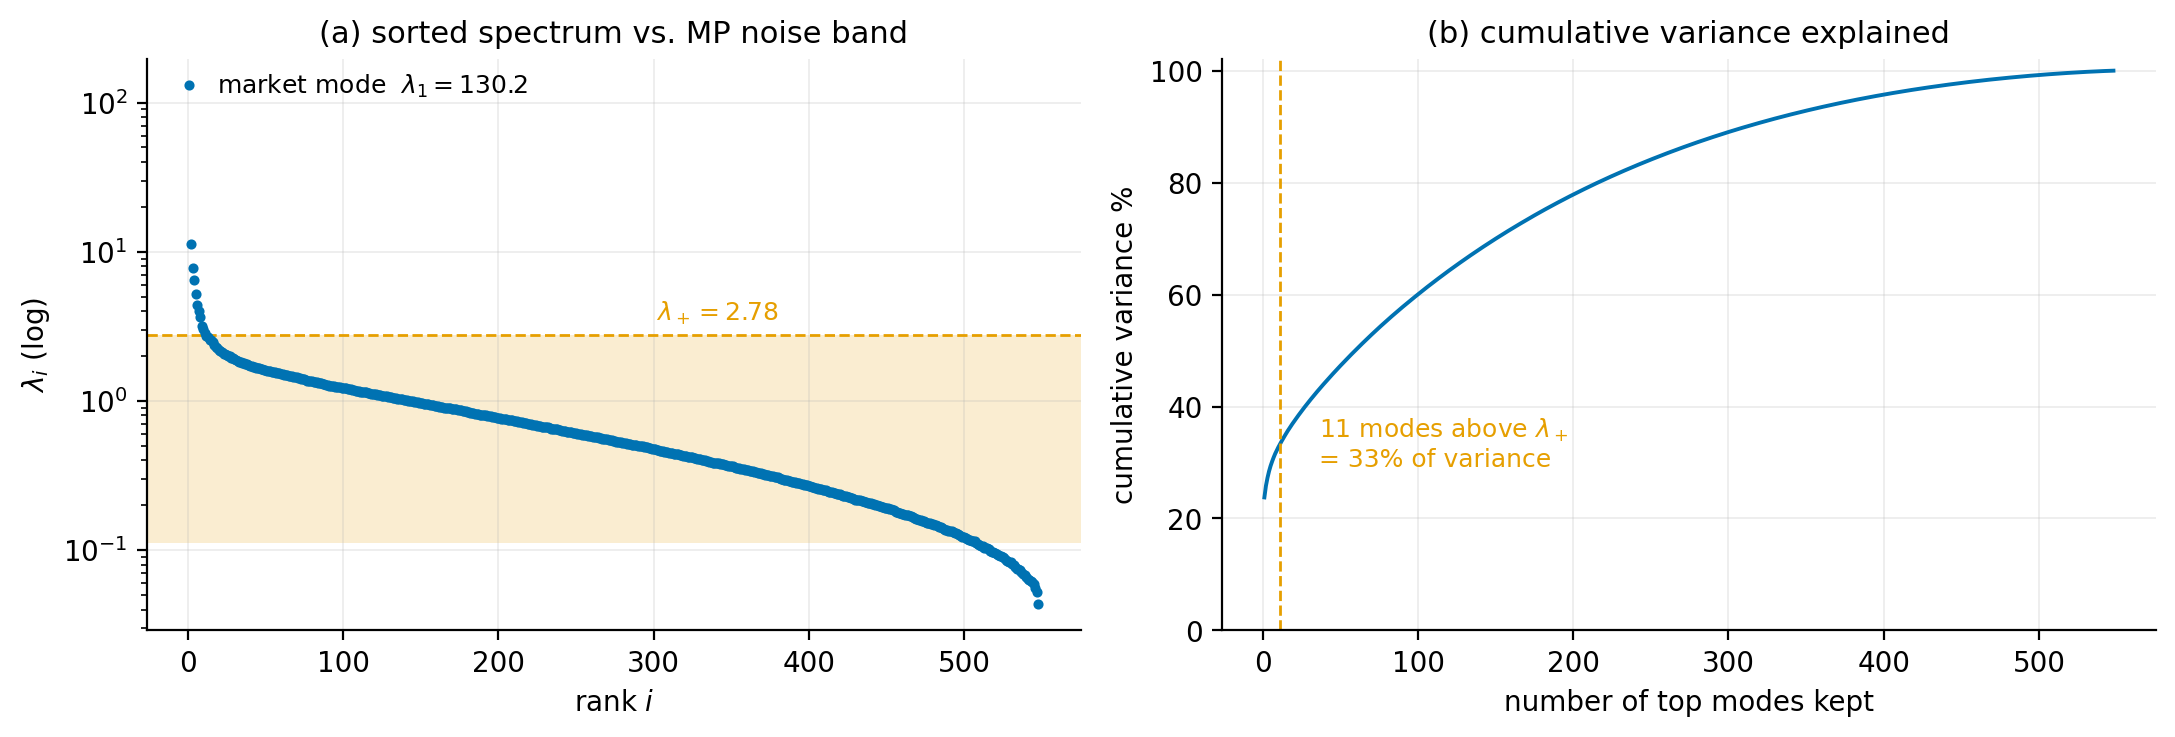
\includegraphics[width=\textwidth]{fig_phase1_spectrum.png}
\caption{The spectrum meets the theorem. (a)~Sorted eigenvalues of the NSE
correlation matrix against the $\sigma^2=1$ Marchenko--Pastur band
(shaded): the bulk hugs the band; 11 eigenvalues escape above, led by the
market mode $\lambda_1=130$. (b)~Those few escapees carry a third of all
variance.}
\label{fig:spectrum}
\end{figure}

\begin{figure}[t]
\centering
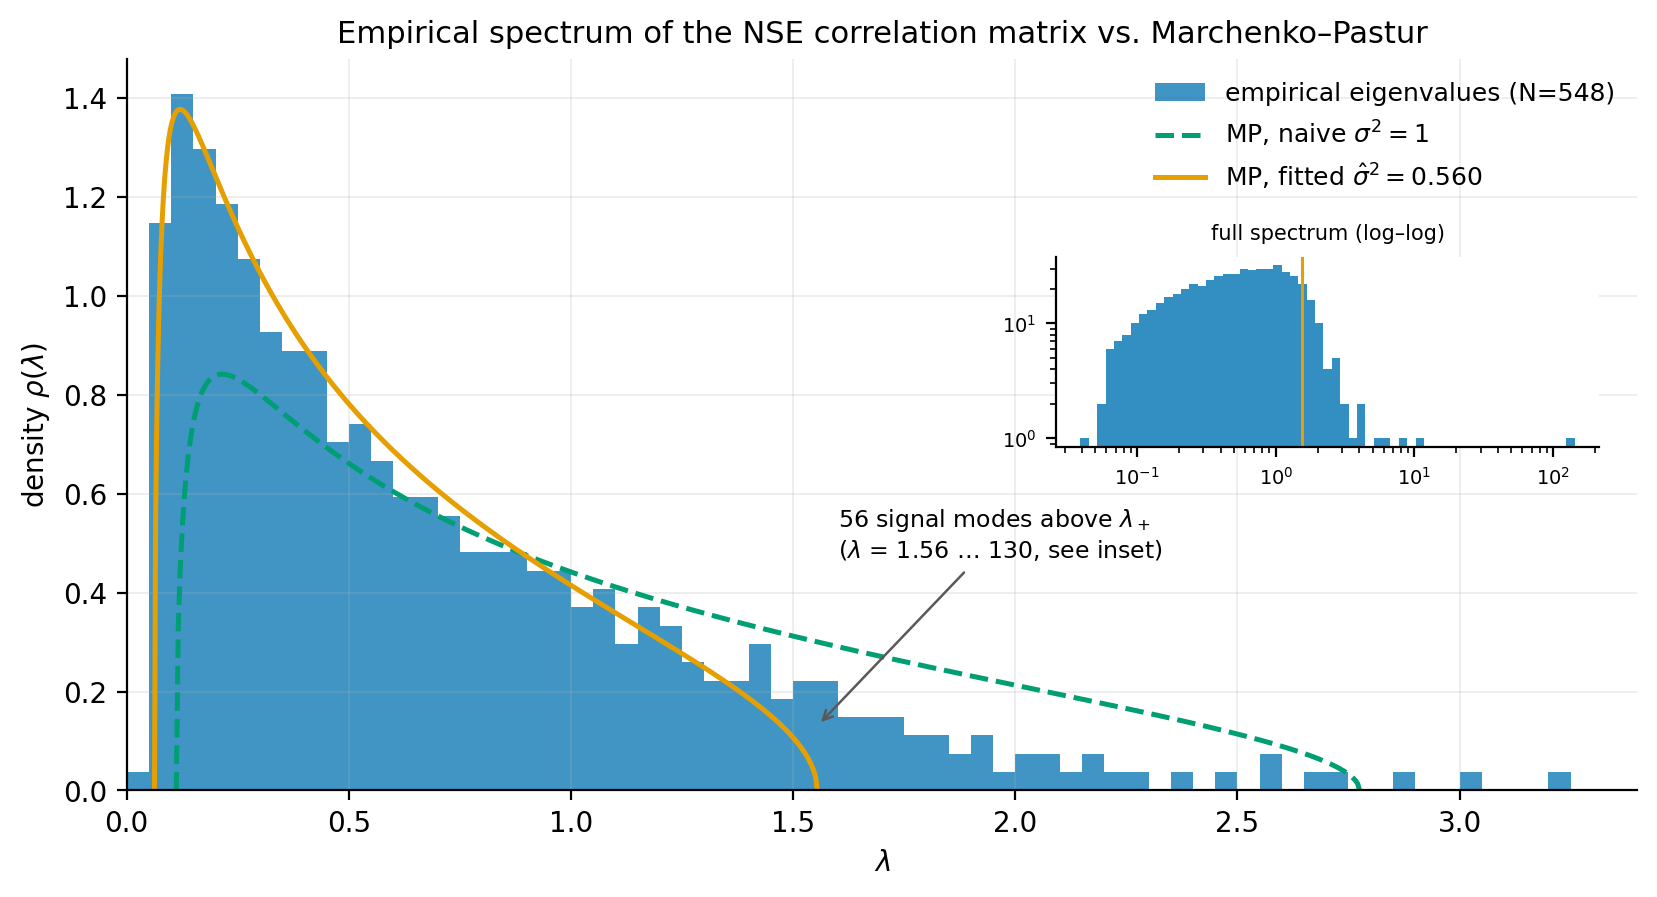
\includegraphics[width=0.92\textwidth]{fig_phase2_mp_density.png}
\caption{The global test: eigenvalue histogram against the
Marchenko--Pastur density, Eq.~\eqref{eq:mpdensity}. The naive
$\sigma^{2}=1$ curve (dashed) is too wide because the signal modes absorb a
third of the trace; with the effective bulk variance fitted
($\hat\sigma^{2}=0.560$, solid) the law tracks the data closely
(Kolmogorov--Smirnov distance $0.024$). Inset: full spectrum, log--log.}
\label{fig:mp}
\end{figure}

\subsection{The global test: the eigenvalues sit where noise sits}

With $\gamma=0.443$ the noise
band is $[0.11,2.78]$. Figure~\ref{fig:spectrum} shows what five years of
Indian equities actually produce: 496 of 548 eigenvalues (90.5\%) inside
the band; 11 above it, led by $\lambda_1=130.2$---the market mode, whose
eigenvector weights all 548 stocks with the same sign and which alone
carries 23.8\% of total variance. Comparing the bulk's \emph{shape} to
Eq.~\eqref{eq:mpdensity} requires one refinement from the applied
literature \cite{laloux1999}: the signal modes absorb a third of the
trace, so the noise bulk lives on the remaining two-thirds and its
effective variance is below one. Fitting $\sigma^{2}$ gives
$\hat\sigma^{2}=0.560$, and Figure~\ref{fig:mp} shows the result: the MP
density tracks the empirical bulk closely.

\begin{figure}[t]
\centering
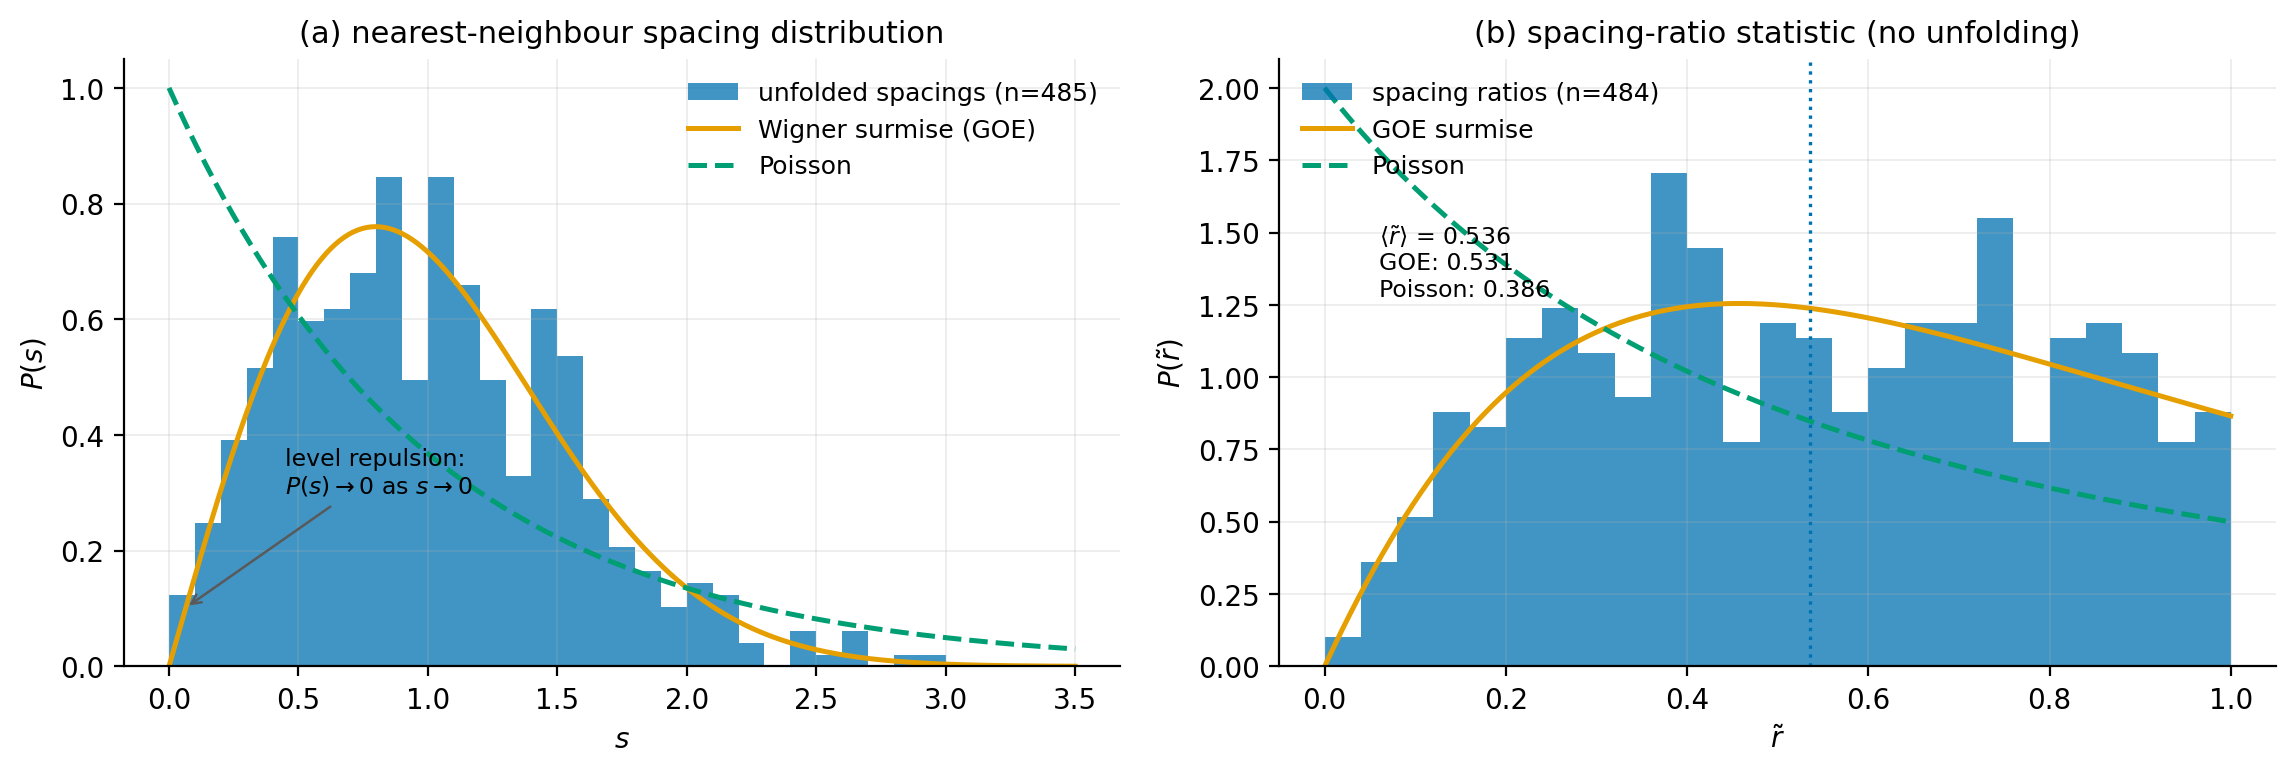
\includegraphics[width=\textwidth]{fig_phase3_spacing.png}
\caption{The local test: Wigner's surmise on real data. (a)~Distribution
of spacings between adjacent noise-band eigenvalues (unfolded to unit mean
spacing) against Eq.~\eqref{eq:surmise} and the Poisson alternative: the
data show exactly the level repulsion of Section~\ref{sec:surmise}.
(b)~The spacing-ratio statistic, which requires no unfolding, agrees:
$\langle\tilde r\rangle=0.536$ against the GOE value $0.531$ and the
Poisson value $0.386$.}
\label{fig:spacing}
\end{figure}

\subsection{The local test: the eigenvalues repel the way noise repels}

The density is a global
statement, and Section~\ref{sec:wigner} taught that random matrices make a
second, sharper promise: level repulsion. So I tested it. Take the 486
eigenvalues inside the fitted band, unfold them (rescale so the local mean
spacing is one, using the fitted MP law as the density), and histogram the
485 adjacent spacings. Figure~\ref{fig:spacing} shows the result against
the two candidates of Section~\ref{sec:surmise}: the data follow Wigner's
surmise---the same curve derived from the $2\times2$ matrix---and reject
the Poisson alternative decisively (Kolmogorov--Smirnov distance $0.027$
against the surmise, versus $0.209$ against Poisson; compared with noise
simulations of matching size, the surmise is fully consistent while
Poisson is excluded at eleven standard deviations). The unfolding-free
ratio statistic $\tilde r_i=\min(s_i,s_{i+1})/\max(s_i,s_{i+1})$
\cite{oganesyan2007} agrees: $\langle\tilde r\rangle=0.536$, against
$0.531$ for GOE and $0.386$ for Poisson. The noise band does not merely
\emph{sit} where the Marchenko--Pastur theorem says noise sits; its
eigenvalues \emph{repel} exactly as Wigner said noise eigenvalues repel.
Both layers of the theory hold in this market, and together they license
what comes next.

\subsection{The economic test: does the noise band price like noise?}
\label{sec:backtest}

The two spectral tests certify that the band \emph{looks} like noise.
They cannot certify that it is \emph{useless}: a curve can fit
beautifully and still hide a sliver of real, exploitable information.
So the final test leaves curve-fitting behind and stakes money---
simulated money, but scored with complete honesty---on the answer.

Here is the experiment in plain terms. We do something deliberately
drastic to the covariance matrix: keep the handful of eigenvalues that
stick out above the noise band (about eleven of 548, in a typical year
of data), and \emph{erase every distinction} the data drew among the
hundreds of directions inside it, replacing them all by one flat
average level---chosen so that total variance is preserved: we
reattribute risk, we never delete it. Now ask what this act of vandalism
does to real portfolios. If the band contains genuine information about
risk, destroying it must make our portfolios \emph{worse}. If the band
is noise, then the ``information'' we erased was never information at
all---it was the statistical equivalent of static---and erasing it
should actually \emph{help}, because the portfolio optimizer will no
longer be fooled by it. Both outcomes are possible in advance. The
future decides. (One case is settled before the race begins: with one
year of data---252 days---and 548 stocks, the raw covariance matrix
breaks down completely, like trying to pin down 548 unknowns from 252
equations. The cleaned matrix has no such problem: filling in the noise
floor is exactly what repairs it.)

The test is run as a four-year contest between four imaginary fund
managers. Each has the same mandate---hold the least-risky fully
invested portfolio you can build, Eq.~\eqref{eq:gmv}---and each sees
only the past, never the future. Once a month, every manager
re-estimates risk from the trailing window of returns and rebalances;
the portfolio is then held for the next month, whose returns none of
them has seen, and its day-by-day performance is recorded. The four
differ only in how they treat the covariance matrix.
\textbf{Manager~1 (raw)} trusts the estimate exactly as it comes (using
the standard mathematical workaround, a pseudo-inverse, when it breaks).
\textbf{Manager~2 (MP-cleaned)} erases the noise band, as above, with
the threshold set purely from past data.
\textbf{Manager~3 (Ledoit--Wolf)} applies the standard statistical
remedy \cite{ledoit2004}: nudge every eigenvalue toward the
average---cautious and sensible, but blind, with no theory of which
eigenvalues are noise.
\textbf{Manager~4 (equal weight)} ignores covariances entirely and
splits the money evenly across all 548 stocks---the famously
hard-to-beat benchmark \cite{demiguel2009}. Every trade is charged a
realistic transaction cost. Because the mandate is low risk, the score
is simple: \emph{how bumpy was each manager's ride}---the realized
volatility of each portfolio over roughly a thousand days of unseen
data. To make sure nothing hinges on an arbitrary choice, the whole
contest is run twice, once with a one-year estimation window and once
with three years. Table~\ref{tab:backtest} and
Figure~\ref{fig:backtest} report both runs.

\begin{table}[t]
\centering
\caption{Out-of-sample minimum-variance performance, NSE equities.
Annualized volatility and return in percent; Sharpe net of 10\,bps costs;
turnover one-way per rebalance; leverage is average $\sum_i|w_i|$.
Top: $T_{\mathrm{est}}=252$ (47 rebalances, Jul 2022--Jun 2026; raw matrix
singular, pseudo-inverted). Bottom: $T_{\mathrm{est}}=756$ (23 rebalances,
Jul 2024--Jun 2026; raw invertible).}
\label{tab:backtest}
\small
\begin{tabular}{lrrrrr}
\toprule
 & Ann.\ vol & Ann.\ ret & Sharpe (net) & Turnover & Leverage \\
\midrule
\multicolumn{6}{l}{\emph{$T_{\mathrm{est}}=252$}}\\
Raw (pseudo-inverse) & 19.37 & 24.67 & 0.93 & 5.36 & 6.86 \\
MP-cleaned & \textbf{7.81} & 13.57 & 1.61 & 0.84 & 2.79 \\
Ledoit--Wolf & 9.29 & 16.64 & 1.57 & 1.67 & 3.83 \\
Equal weight & 17.66 & 29.27 & 1.65 & 0.07 & 1.00 \\
\midrule
\multicolumn{6}{l}{\emph{$T_{\mathrm{est}}=756$}}\\
Raw & 13.01 & $-8.21$ & $-0.94$ & 3.50 & 7.95 \\
MP-cleaned & \textbf{8.87} & $-4.81$ & $-0.62$ & 0.64 & 3.24 \\
Ledoit--Wolf & 10.23 & $-3.71$ & $-0.55$ & 1.65 & 5.28 \\
Equal weight & 19.36 & 6.61 & 0.34 & 0.07 & 1.00 \\
\bottomrule
\end{tabular}
\end{table}

\begin{figure}[t]
\centering
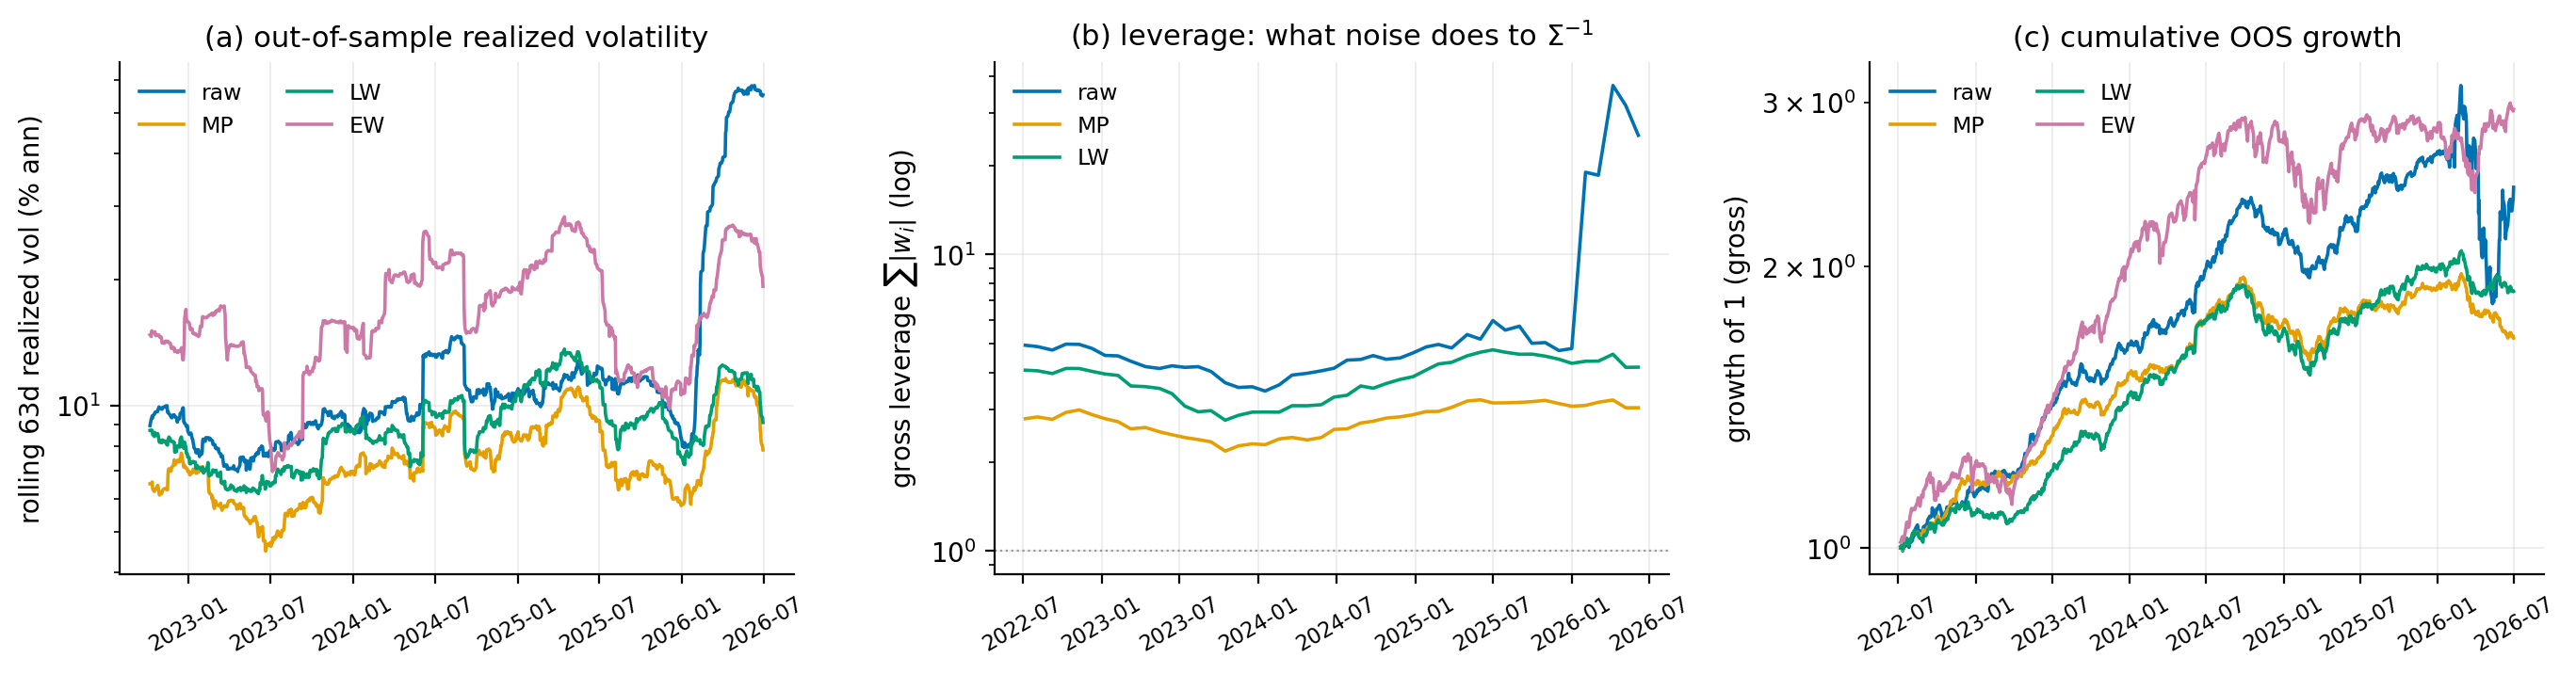
\includegraphics[width=\textwidth]{fig_phase7_backtest.png}
\caption{The backtest through time ($T_{\mathrm{est}}=252$). (a)~Rolling
realized volatility: the MP-cleaned portfolio is lowest almost throughout.
(b)~Gross leverage: the raw matrix's noise-driven bets spike to
${\sim}40\times$ in early 2026, exactly when its realized risk explodes.
(c)~Cumulative out-of-sample growth.}
\label{fig:backtest}
\end{figure}

The contest is not close. Manager~1, who trusted everything the sample
said, had the wildest ride: 19.4\% annualized volatility---worse than
ignoring covariances altogether. The reason is visible in
Figure~\ref{fig:backtest}b, and it is the error maximization of
Section~\ref{sec:wishart} caught on camera. The noisy matrix keeps
``discovering'' combinations of stocks that look magically safe, and the
optimizer piles into them: for every rupee of capital, Manager~1 holds
about seven rupees of offsetting long and short positions on average,
spiking to nearly \emph{forty} in early 2026---precisely when the
portfolio's realized risk explodes. Those magically safe combinations
were mirages of sampling error, and they evaporated in the very next
month, month after month, forcing frantic, expensive trading to chase
their replacements. Manager~2, who erased the noise band, had the
calmest ride of all four: 7.81\%---less than half the raw manager's
risk---achieved with modest positions and the least trading of any
covariance-based strategy. Manager~3's blind shrinkage helped
(9.29\%) but gave up a meaningful gap to Manager~2 while trading twice
as much; Manager~4's equal weights realized 17.7\%. And the gaps are
far too large to be luck: a standard statistical comparison of
day-by-day risk (a Diebold--Mariano test) puts the odds that chance
alone explains Manager~2's edge over Managers~3 and~4 below one in ten
thousand, and below one in six hundred against Manager~1. The second
run of the contest, with three-year windows---where the raw matrix works
without any mathematical workaround---produces the same finishing order
(8.87\% vs.\ 10.23\% vs.\ 13.01\%), so nothing here is an artifact of
the one-year window. Even after trading costs, Manager~2 has the best
risk-adjusted performance of the three covariance-based strategies.

Pause on how strange this result would be if the band were not noise.
Manager~2 threw away 98\% of the distinctions in the estimated
matrix---the most destructive thing a manager could do to their own
risk model---and \emph{won because of it}. Had the band contained real
information, that act would have placed Manager~2 last, not first: the
experiment was completely free to falsify the noise hypothesis, and
instead it confirmed it. The three layers of evidence now interlock.
The band's eigenvalues are \emph{distributed} like noise
(Figure~\ref{fig:mp}); they \emph{interact} like noise
(Figure~\ref{fig:spacing}); and---the strictest test, because it risks
being wrong about the future---they \emph{price} like noise: portfolios
that discard them beat portfolios that trust them, portfolios that
shrink them blindly, and portfolios that ignore covariances altogether.
The noise band is legit. (The fine print, stated honestly: the stock
list is today's index membership, so the sample tilts toward companies
that survived---a bias that affects all four managers identically; the
portfolios are unconstrained and long--short, the setting where the
quality of a covariance matrix matters most; trading costs are
stylized; and this is one market over one five-year period.)

\section{Conclusion: what I learned}
\label{sec:conclusion}

Three things, in ascending order of surprise. First, the classical theory
is a single connected story: Wigner's move---model ignorance as
randomness, then compute what is universal---transfers from nuclear
Hamiltonians to sample covariance matrices with only a change of ensemble,
from GOE to Wishart, and a change of limiting spectral law, to
Marchenko--Pastur; the proofs themselves are assembled from a small kit
(a transform that smooths the spectrum, a rank-one update, a determinant
identity, a concentration estimate) whose members are each elementary.
Second, the limit $N,T\to\infty$ at fixed $\gamma=N/T$ is not an analyst's
convenience but the entire content of the modern viewpoint: $\gamma$ is
the price of estimation measured in parameters per datum, the classical
theory is the $\gamma\to0$ edge of the family, and real datasets live well
inside it. Third---and this was not obvious to me before doing it---the
theory is \emph{quantitatively} true of a real emerging market: five years
of NSE returns produce a spectral bulk with the Marchenko--Pastur shape
and Wigner's level repulsion, and acting on that diagnosis, by the
simplest possible filter, beats both the raw estimate and the standard
shrinkage remedy out of sample, by a wide and statistically significant
margin. Random matrix theory begins as a confession of ignorance; applied
carefully, it ends as an instrument precise enough to trust with money.

\begin{thebibliography}{12}

\bibitem{wigner1958}
E.~P. Wigner,
On the distribution of the roots of certain symmetric matrices,
\emph{Annals of Mathematics} \textbf{67}, 325--327 (1958).

\bibitem{mehta2004}
M.~L. Mehta,
\emph{Random Matrices}, 3rd ed., Elsevier, Amsterdam (2004).

\bibitem{wishart1928}
J.~Wishart,
The generalised product moment distribution in samples from a normal
multivariate population,
\emph{Biometrika} \textbf{20A}, 32--52 (1928).

\bibitem{marchenko1967}
V.~A. Mar\v{c}enko and L.~A. Pastur,
Distribution of eigenvalues for some sets of random matrices,
\emph{Mathematics of the USSR-Sbornik} \textbf{1}, 457--483 (1967).

\bibitem{baisilverstein2010}
Z.~Bai and J.~W. Silverstein,
\emph{Spectral Analysis of Large Dimensional Random Matrices}, 2nd ed.,
Springer, New York (2010).

\bibitem{laloux1999}
L.~Laloux, P.~Cizeau, J.-P. Bouchaud, and M.~Potters,
Noise dressing of financial correlation matrices,
\emph{Physical Review Letters} \textbf{83}, 1467--1470 (1999).

\bibitem{plerou2002}
V.~Plerou, P.~Gopikrishnan, B.~Rosenow, L.~A.~N. Amaral, T.~Guhr, and
H.~E. Stanley,
Random matrix approach to cross correlations in financial data,
\emph{Physical Review E} \textbf{65}, 066126 (2002).

\bibitem{bun2017}
J.~Bun, J.-P. Bouchaud, and M.~Potters,
Cleaning large correlation matrices: tools from random matrix theory,
\emph{Physics Reports} \textbf{666}, 1--109 (2017).

\bibitem{oganesyan2007}
V.~Oganesyan and D.~A. Huse,
Localization of interacting fermions at high temperature,
\emph{Physical Review B} \textbf{75}, 155111 (2007).

\bibitem{michaud1989}
R.~O. Michaud,
The Markowitz optimization enigma: is `optimized' optimal?,
\emph{Financial Analysts Journal} \textbf{45}(1), 31--42 (1989).

\bibitem{demiguel2009}
V.~DeMiguel, L.~Garlappi, and R.~Uppal,
Optimal versus naive diversification: how inefficient is the $1/N$
portfolio strategy?,
\emph{Review of Financial Studies} \textbf{22}, 1915--1953 (2009).

\bibitem{ledoit2004}
O.~Ledoit and M.~Wolf,
A well-conditioned estimator for large-dimensional covariance matrices,
\emph{Journal of Multivariate Analysis} \textbf{88}, 365--411 (2004).

\end{thebibliography}

\end{document}
